\documentclass[11pt,a4paper]{report}
\usepackage[utf8]{inputenc}
\usepackage[portuguese]{babel}
\usepackage[T1]{fontenc}
\usepackage{amsmath}
\usepackage{amsfonts}
\usepackage{amssymb}
\usepackage{graphicx}
\usepackage[hmargin=2cm,vmargin=3.5cm,bmargin=2cm]{geometry}
\usepackage{color} 
\usepackage{csquotes}
\usepackage{hyperref}
\hypersetup{
    colorlinks=true, %set true if you want colored links
    linktoc=all,     %set to all if you want both sections and subsections linked
    linkcolor=blue,  %choose some color if you want links to stand out
}

\usepackage{listings}
\usepackage{xcolor}

\definecolor{codegreen}{rgb}{0,0.6,0}
\definecolor{codegray}{rgb}{0.5,0.5,0.5}
\definecolor{codepurple}{rgb}{0.58,0,0.82}
\definecolor{backcolour}{rgb}{0.95,0.95,0.92}

\lstdefinestyle{mystyle}{
    backgroundcolor=\color{backcolour},   
    commentstyle=\color{codegreen},
    keywordstyle=\color{magenta},
    numberstyle=\tiny\color{codegray},
    stringstyle=\color{codepurple},
    basicstyle=\ttfamily\footnotesize,
    breakatwhitespace=false,         
    breaklines=true,                 
    captionpos=b,                    
    keepspaces=true,                 
    numbers=left,                    
    numbersep=5pt,                  
    showspaces=false,                
    showstringspaces=false,
    showtabs=false,                  
    tabsize=2
}

\lstset{style=mystyle}

\author{Gonçalo Teixeira e Gonçalo Alves}
\title{Redes de Computadores - 2.º Trabalho}
\graphicspath{ {pictures/} }

\begin{document}
\begin{titlepage}
    \begin{center}
        \vspace*{1cm}
            
        \Huge
        \textbf{Redes de Computadores}
            
        \vspace{0.5cm}
        \LARGE
        2.º Trabalho Prático - Rede de Computadores
            
        \vspace{1.5cm}
            
        \textbf{Gonçalo Teixeira e Gonçalo Alves}
            
        \vfill
            
       	Mestrado Integrado em Engenharia\\
       	Informática e Computação
            
        \vspace{0.8cm}
            
        
\includegraphics[width=0.4\textwidth]{uporto-feup}
        
        \Large
        \today\\
        Porto
       	 
    \end{center}
\end{titlepage}

\cleardoublepage
\phantomsection
\addcontentsline{toc}{section}{Sumário}
\section*{Sumário}
Sumário aqui -> dizer para que é que serve este relatório

%Índice de conteúdos
\tableofcontents 

% Body
\cleardoublepage
\phantomsection
\addcontentsline{toc}{section}{Introdução}
\section*{Introdução}
Este trabalho é composto por duas partes, tal como foi mencionado no sumário, a primeira parte consiste no desenvolvimento de uma aplicação de \emph{download}; a segunda parte consiste na configuração e estudo de uma rede de computadores.

\noindent A rede configurada deve ser capaz de permitir a execução da aplicação \emph{download} com sucesso, além disso, deve contemplar duas vlans dentro de um Cisco Switch, a configuração de um Cisco Router e implementação de NAT e DNS.

\noindent Este relatório está também subdivido em duas partes principais, a exposição teórica do processo de desenvolvimento e teste da aplicação \emph{download}, e para segunda parte, percorrer-se-à a configuração da rede experiência a experiência, respondendo a cada pergunta colocada no guião, acompanhado com figuras e registos.

\noindent Depois da exposição teórica do assunto e do desenvolvimento, apresentar-se-ão conclusões acerca dos objetivos propostos e conhecimentos adquiridos.

\cleardoublepage
\phantomsection
\addcontentsline{toc}{section}{Parte I - Aplicação Download}
\section*{Parte I - Aplicação Download}
A primeira parte deste segundo trabalho foi o desenvolvimento de uma aplicação de download, que requere
um link do tipo ftp://[<user>:<password>@]<host>/<url-path> (tal como descrito em RFC1738), através de um servidor FTP.

\addcontentsline{toc}{subsection}{Arquitetura}
\subsection*{Arquitetura}
Numa fase inicial é feito o \textit{parsing} do link passado como argumento.
A função \textit{parseArg} recolhe os devidos campos (\textit{user},\textit{password},\textit{host} e \textit{url\char`_path}), e guarda nas variáveis com o mesmo nome.
No caso dos campos \textit{user} e \textit{password} não estarem presentes no link, serão dados os valores de \textit{anonymous} e \textit{1234}, respetivamente.

De seguida, através de código já fornecido pelos docentes, é obtido o \textit{IP address}, usando a função \textit{getIP(host)}.

Após estes passos, é iniciada a conexão entre o cliente e o servidor, através da abertura de um \textit{socket} (\textit{socket\char`_connection}, adaptado do código disponibilizado pelos docentes).
É necessário referir que a partir desta conexão, a comunicação entre cliente-servidor é muito semelhante para os diferentes comandos enviados: é feita com base no envio de pedidos (\textit{ftp\char`_write\char`_socket}, retorna 0 se o envio foi bem sucedido, -1 em contrário) e leitura de respostas (\textit{ftp\char`_read\char`_socket}, retorna o código de resposta do servidor). Como tal, quando for referido o envio de um comando, na realidade está-se a querer dizer o envio de um pedido e receção da resposta consequente.
Assim, após a conexão inicial:
\begin{itemize}
\item É verificado se a conexão foi estabelecida(\textit{ftp\char`_init\char`_connection});
\item São enviados os comandos \textbf{USER user}, \textbf{PASS password}, \textbf{TYPE I} de modo a fazer o login (\textit{ftp\char`_login});
\item É enviado o comando \textbf{PASV}, de modo a entrar no modo passivo (\textit{ftp\char`_passive});
\item É aberto um novo \textit{socket}, para troca de dados, é enviado o comando \textbf{RETR url\char`_path} (\textit{ftp\char`_retrieve}), de modo a fazer o pedido do ficheiro, é feito o download do ficheiro (\textit{ftp\char`_get\char`_file}) e são fechados os \textit{sockets} de dados e de comandos (\textit{socket\char`_exit}), terminando a aplicação (\textit{ftp\char`_download}).
\end{itemize}
\addcontentsline{toc}{subsection}{Resultados}
\subsection*{Resultados}
A nossa aplicação foi testada com: modo anónimo, modo autenticado, diferentes tipos de ficheiro, diferentes tamanhos de ficheiros. Em todos os casos, foi bem sucedida.
Durante a execução do programa são apresentadas as informações iniciais (\textit{user},\textit{password},\textit{host}, \textit{$url_path$} e \textit{IP}) e as respostas do servidor, de modo a proporcionar ao utilizador o estado do download. 

\cleardoublepage
\phantomsection
\addcontentsline{toc}{section}{Parte II - Configuração e Análise de Rede}
\section*{Parte II - Configuração e Análise de Rede}
Pequeno texto acerca da rede a configurar

\phantomsection
\addcontentsline{toc}{subsection}{Experiência 1 - Configuração IP de Rede}
\subsection*{Experiência 1 - Configuração IP de Rede}
O objetivo desta experiência é ligar dois tux através de um switch.

\subsubsection{1. O que são os pacotes ARP e para que são usados?}
O ARP (\emph{Address Resolution Protocol}) é um protocolo de comunicação que serve para descobrir o endereço da camada de ligação associado ao endereço IP numa LAN (\emph{Local Area Network}). O endereço da camada de ligação é também conhecido por Endereço MAC (\emph{Media Access Control}).

\subsubsection{2. Quais são os endereços MAC e IP dos pacotes ARP e porquê?}
Executando o comando \emph{ping} do tux3 para o tux4, o tux3 envia uma pergunta para saber qual é o endereço MAC associado ao IP do tux4. A \enquote{pergunta} é feita através de um pacote ARP que contém o endereço IP e MAC do tux3 (\verb+172.16.30.1+ e \verb+00:21:5a:5a:7d:74+) e o endereço IP do tux4 (\verb+172.16.1.254+), uma vez que se quer descobrir o endereço MAC do tux4, o campo dedicado a esse efeito está a \verb+00:00:00:00:00:00+. De seguida é enviada uma resposta, também sob a forma de um pacote ARP, do tux4 para o tux3, indicando o seu endereço MAC (\verb+00:21:5a:5a:7d:74+). Figura \ref{fig:fig1}

\subsubsection{3. Quais os pacotes gerados pelo comando ping?}
Primeiro o comando \emph{ping} gera pacotes ARP para fazer a relação entre endereços IP e MAC, de seguida gera pacotes ICMP (\emph{Internet Control Message Protocol}).

\subsubsection{4. Quais são os endereços MAC e IP dos pacotes ping?}
Quando se executa o comando \emph{ping} no tux3 para o tux4, os endereços (IP e MAC) vão ser os endereços dos tux. Podemos ver de seguida os endereços registados nos pacotes de pedido e reposta, respetivamente.

\begin{table}[ht]
\begin{center}
 	\begin{tabular}{|| c | c c c||} 
 		\hline
 		& tux & MAC & IP \\ [0.5ex] 
 		\hline\hline
 		Origem & 3 & 00:21:5a:61:24:92 & 172.16.30.1 \\ 
 		\hline
 		Destino & 4 & 00:21:5a:5a:7d:74 & 172.16.30.254 \\ [1ex] 
 		\hline
	\end{tabular}
	\caption{Pacote de Pedido}
	\label{tab:table1}
\end{center}
\end{table}

\begin{table}[ht]
\begin{center}
 	\begin{tabular}{|| c | c c c||} 
 		\hline
 		& tux & MAC & IP \\ [0.5ex] 
 		\hline\hline
 		Origem & 4 & 00:21:5a:5a:7d:74 & 172.16.30.254 \\ 
 		\hline
 		Destino & 3 & 00:21:5a:61:24:92 & 172.16.30.1 \\ [1ex] 
 		\hline
	\end{tabular}
	\caption{Pacote de Resposta}
	\label{tab:table2}
\end{center}
\end{table}

Devem-se consultar as figuras \ref{fig:fig2} e \ref{fig:fig3} para referência.

\subsubsection{5. Como determinar se a trama recetora Ethernet é ARP, IP, ICMP?}
O \emph{Ethernet Header} de um pacote contém a informação acerca do tipo da trama. Para as tramas IP, o valor do tipo será \verb+0x0800+, se o \emph{IP Header} tiver o valor 1 então o tipo de protocolo é ICMP. Para as tramas ARP o valor do tipo será \verb+0x0806+.\\
Para referência devem-se consultar as figuras \ref{fig:fig4} e \ref{fig:fig5}.

\subsubsection{6. Como determinar o comprimento de uma trama recetora?}
O  comprimento  de  uma  trama recetora pode ser determinado inspecionando a entrada no registo do \emph{Wireshark}, tal como se pode observar na figura \ref{fig:fig6}.

% Criar os ficheiros devidos e descomentar as linhas
% bloco a bloco

%\phantomsection
%\addcontentsline{toc}{subsection}{Experiência 2 - Implementar duas LANs Virtuais no Switch}
\subsection*{Experiência 2 - Implementar duas LANs Virtuais no Switch}
Explicar sucintamente o objetivo desta experiência.

\subsubsection{1. Como configurar a VLANy0?}
Primeiro é necessário ligar um cabo série do tux3 ao switch para aceder ao terminal de configuração (\emph{configure terminal}) do switch. De seguida cria-se uma vlan, de ID y0, no caso, 31. Por fim resta atribuir as portas em questão a essa vlan que acabou de ser criada.
\begin{lstlisting}[language=bash]
configure terminal
> vlan y0
> end
> configure terminal
> interface fastethernet 0/[n da porta]
> switchport mode access
> switchport access vlan y0
> end

\end{lstlisting}

\subsubsection{2. Quantos domínios de broadcast existem? O que se pode concluir a partir dos registos?}
O tux3 recebe resposta do tux4 quando faz \emph{ping boradcast}, mas não recebe do tux2. O tux2 não recebe nenhuma resposta quando executa a instrução de \emph{ping broadcast}. Desta forma pode-se concluir que existem dois domínios de broadcast, um que contem o tux3 e tux4, e outro que contém o tux2.


%\phantomsection
%\addcontentsline{toc}{subsection}{Experiência 3 - Configurar um Router em Linux}
\subsection*{Experiência 3 - Configurar um Router em Linux}
O objetivo desta experiência é configurar um tux para servir de router e transmitir dados da uma vlan para outra.

\subsubsection{1. Que rotas existem nos tux? Qual o seu significado?}
\begin{table}[ht]
\begin{center}
 	\begin{tabular}{|| c c c||} 
 		\hline
 		tux & vlan & gateway \\ [0.5ex] 
 		\hline\hline
 		2 & vlan0 172.16.y0.0 & 172.16.y1.253\\ 
 		\hline
 		2 & vlan1 172.16.y1.0 & 0.0.0.0\\ 
 		\hline\hline
 		3 & vlan0 172.16.y0.0 & 0.0.0.0\\ 
 		\hline
 		3 & vlan1 172.16.y1.0 & 172.16.y1.254\\ 
 		\hline\hline
 		4 & vlan0 172.16.y0.0 & 0.0.0.0\\ 
 		\hline
 		4 & vlan1 172.16.y1.0 & 0.0.0.0\\ [1ex] 
 		\hline
	\end{tabular}
	\caption{Rotas Existentes nos tux}
	\label{tab:table3}
\end{center}
\end{table}

O destino das rotas é até onde o tux que está na origem da rota consegue chegar.

\subsubsection{2. Qual é a informação que uma entrada da tabela de \emph{forwarding} contém?}
\textbf{\emph{Destination}}: o destino da rota;\\
\textbf{\emph{Gateway}}: o IP do próximo ponto por onde passará a rota;\\
\textbf{\emph{Netmask}}: usado para determinar o ID da rede a partir do endereço IP do destino;\\
\textbf{\emph{Flags}}: informações sobre a rota;\\
\textbf{\emph{Metric}}: o custo de cada rota;\\
\textbf{\emph{Ref}}: número de referências para esta rota (não usado no kernel do Linux);\\
\textbf{\emph{Use}}: contador de pesquisas pela rota, dependendo do uso de -F ou -C isto vai ser o número de falhas da cache (-F) ou o número de sucessos (-C);\\
\textbf{\emph{Interface}}: qual a placa de rede responsável pela gateway (\emph{eth0}/\emph{eth1}).

\subsubsection{3. Que mensagens ARP e endereços MAC associados são observados e porquê?}
Tal como referido nos pontos 1 e 2 da experiência 1, quando um tux faz \emph{ping} para outro tux é preciso relacionar o IP do destino com um endereço MAC. Podem ser consultadas a figuras \ref{fig:fig7} (eth1 tux4) e \ref{fig:fig8} (eth0 tux4).

\subsubsection{4. Que pacotes ICMP são observados e porquê?}
São observados pacotes de pedido e resposta ICMP, uma vez que as rotas estão configuradas, caso contrário seriam enviados pacotes ICMP de \emph{Host Unreachable}. Pode ser consultada a figura \ref{fig:fig9} para referência.

\subsubsection{5. Quais são os endereços IP e MAC associados a um pacote ICMP e porquê?}
Os endereços IP e MAC associados com os pacotes ICMP são os endereços IP e MAC dos tux de origem e destino. Quando é feito \emph{ping} do tux3 para o tux4 os endereços de origem vão ser \verb+172.16.y0.1+ (IP) e \verb+00:21:5a:61:24:92+ (MAC) e o de destino \verb+172.16.y1.253+ (IP) e \verb+00:21:5a:5a:7d:74+ (MAC).


%\phantomsection
%\addcontentsline{toc}{subsection}{Experiência 4 - Configurar um Router comercial e implementar o NAT}
\subsection*{Experiência 4 - Configurar um Router comercial e implementar o NAT}
O objetivo desta experiência é configurar um Router comercial e configurar o serviço NAT para acesso à Internet.

\subsubsection{1. Como se configura um Router estático num Router comercial?}
Para configurar o Router é necessário ligar um cabo série do tux ao router, depois executam-se os seguintes comandos no \emph{GTKTerm} (router):

\begin{lstlisting}[language=bash]
	configure terminal
	> ip route [destino] [mascara] [gateway]
	> exit
\end{lstlisting}

\subsubsection{2. Quais são as rotas seguidas pelos pacotes durante a experiência? Explique.}
No caso de a rota existir, os pacotes utilizam essa rota, caso contrário, os pacotes passam pela rota default (router), são informados que o tux4 existe, e deverão ser enviados pelo mesmo.

\subsubsection{3. Como se configura o NAT num Router comercial?}
Para configurar o router, foi necessário configurar a interface interna no processo de NAT, o que foi feito recorrendo ao guião fornecido. Ligando ao router através da porta série, utilizamos os seguintes comandos que podem ser consultados em anexo, figura \ref{fig:fig10}.

\subsubsection{4. O que faz o NAT?}
O \emph{Network Address Translation} NAT foi concebido para a preservação de endereços IP. Permite que as redes IP privadas que usem endereços IP não registados a possibilidade de se ligarem à Internet. O NAT opera num router, normalmente ligando duas redes, e traduz os endereços da rede privada (que não são únicos à escala global) em endereços válidos, antes que os pacotes sejam transmitidos para outra rede.
Adicionalmente, o NAT pode ser configurado para mostrar apenas um endereço correspondente à rede privada inteira para a rede exterior. Isto transmite segurança adicional uma vez que esconde de forma eficaz os endereços da rede que está por detrás daquele endereço público. Adicionalmente, o NAT oferece também funções de segurança e é implementado em
ambientes de acesso remoto.\\
Resumidamente, o NAT permite que os computadores de uma rede interna tenham acesso ao exterior, sendo que, um único endereço IP é exigido para representar um grupo de computadores fora da sua própria rede. 



%\phantomsection
%\addcontentsline{toc}{subsection}{Experiência 5 - DNS}
\subsection*{Experiência 5 - DNS}
Explicar sucintamente o objetivo desta experiência.

\subsubsection{1. Como configurar um serviço DNS num \emph{host}?}
Para configurar o serviço DNS, é necessário alterar o ficheiro \verb+resolv.conf+ no \emph{host}. Esse ficheiro tem de conter as seguintes linhas:
\begin{lstlisting}[language=bash]
	search netlab.fe.up.pt
	nameserver 172.16.1.1
\end{lstlisting}

Em que \verb+netlab.fe.up.pt+ é o nome do servidor DNS e \verb+172.16.1.1+ é o seu endereço IP. Após esta experiência é possível fazer \emph{ping} a \verb+google.com+ com sucesso e, portanto, aceder à Internet nos tux.

\subsubsection{2. Que pacotes são trocados pelo DNS e que informações são transportadas?}
São trocados pacotes de protocolo DNS, em que o \emph{host} pede ao servidor de DNS o IP associado ao nome que indicou, por exemplo \verb+ftp.up.pt+, e o servidor depois responde com o endereço IP associado. Pode ser consultada a figura \ref{fig:fig11} para referência. 


%\phantomsection
%\addcontentsline{toc}{subsection}{Experiência 6 - Ligações TCP}
\subsection*{Experiência 6 - Ligações TCP}
O objetivo desta experiência é analisar como funcionam as ligações TCP e inspecionar o funcionamento da aplicação \emph{download} desenvolvida.

\subsubsection{1. Quantas ligações TCP foram abertas pela aplicação FTP?}
A aplicação abriu duas ligações TCP, uma para enviar comandos e receber respostas do servidor e 
uma outra para receber dados do servidor e enviar as repostas do cliente.

\subsubsection{2. Em que ligação é transportado a informação de controlo?}
A informação de controlo é transportada na ligação de troca de comandos, ou seja, na primeira referida no ponto anterior.

\subsubsection{3. Quais são as fases de uma ligação TCP?}
Uma ligação TCP é constituída por 3 fases, uma fase de estabelecimento da ligação, uma fase de troca de dados e uma fase de encerramento da ligação.

\subsubsection{4. Como é que o mecanismo ARQ TCP funciona? Quais os campos TCP relevantes? Qual a informação relevante observada nos registos?}
O TCP utiliza o mecanismo ARQ (\emph{Automatic Repeat Request}) com o método da janela deslizante, que consiste no controlo de erros na transmissão de dados. 
Os campos relevantes para o efeito são os \emph{acknowledgement numbers}, que indicam se a mensagem foi recebida corretamente (recetor); o \emph{window size} que indica a gama de pacotes que o emissor pode enviar e o \emph{sequence number}, que indica o número de sequência do pacote a ser enviado.

\subsubsection{5. Como é que o mecanismo de controlo de congestão TCP funciona? Como é que o fluxo de dados da conexão evoluiu ao longo do tempo? Está de acordo com o mecanismo de controlo de congestão TCP?}
O mecanismo de controlo de congestão é feito quando o TCP mantém uma janela de congestão que consiste numa estimativa do número de octetos que a rede consegue encaminhar, não enviando mais octetos do que o mínimo da janela definida pelo recetor e pela janela de congestão.\\
Ao iniciar a transferência no tux3 registou-se uma subida acentuada no gráfico de fluxo (taxa de transferência), e perto dos 4 segundos, registamos uma descida acentuada da curva do gráfico, seguida de uma estabilização, até terminar. Podemos concluir que ao iniciar a transferência no tux2, a taxa de transferência diminui, o que faz sentido uma vez que o fluxo de dados de ligação está de acordo com o mecanismo de controlo de congestão pois quando a rede estava mais congestionada tinha um bitrate menor. O referido gráfico pode ser consultado na figura \ref{fig:fig12}.

\subsubsection{6. De que forma é afetada a conexão de dados TCP pelo aparecimento de uma segunda conexão TCP? Como?}
Com o aparecimento de uma segunda conexão TCP, a existência de uma transferência de dados em simultâneo pode levar a uma queda na taxa de transmissão, uma vez que a taxa de transferência é distribuída de igualmente. Esta informação pode ser verificada novamente através da figura \ref{fig:fig12}.

\cleardoublepage
\phantomsection
\addcontentsline{toc}{section}{Conclusão}
\section*{Conclusão}
Para conclusão do relatório deste trabalho prático pode-se afirmar que os conceitos relacionados com o funcionamento de uma rede, um elemento presente todos os dias na vida da maioria das pessoas no mundo, foram explorados com sucesso, e portanto, foram interiorizados e consolidados.
\noindent Acerca da aplicação \emph{download} pode-se concluir que foram explorados os conceitos da implementação de um cliente TCP.
\noindent Para conclusão geral deste relatório afirma-se que todos os objetivos foram alcançados, o que contribuiu para um aprofundamento dos conhecimentos teóricos e práticos da Unidade Curricular de Redes de Computadores.

\cleardoublepage
\phantomsection
\addcontentsline{toc}{section}{Referências}
\section*{Referências}

\hypersetup{linkcolor=}

\begin{itemize}
	\item \href{https://www.cisco.com/c/en/us/support/docs/ip/network-address-translation-nat/26704-nat-faq-00.html}{\color{blue}{https://www.cisco.com/c/en/us/support/docs/ip/network-address-translation-nat/26704-nat-faq-00.html}}
	\item \href{https://www.cisco.com/c/en/us/support/docs/ip/domain-name-system-dns/12683-dns-descript.html}{\color{blue}{https://www.cisco.com/c/en/us/support/docs/ip/domain-name-system-dns/12683-dns-descript.html}}
	\item \href{https://www.cisco.com/c/en/us/support/docs/ip/routing-information-protocol-rip/13769-5.html}{\color{blue}{https://www.cisco.com/c/en/us/support/docs/ip/routing-information-protocol-rip/13769-5.html}}
\end{itemize}

\cleardoublepage
\phantomsection
\addcontentsline{toc}{section}{Anexos}
\section*{Anexos}

% incluir as imagens aqui - com label ("Figura X")
\phantomsection
\addcontentsline{toc}{subsection}{Imagens}
\subsection*{Imagens}

\begin{figure}[ht]
	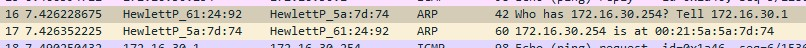
\includegraphics[width=\linewidth]{figure1}                                                      
    \caption{Pacotes ARP}
    \label{fig:fig1}
\end{figure}

\begin{figure}[ht]
	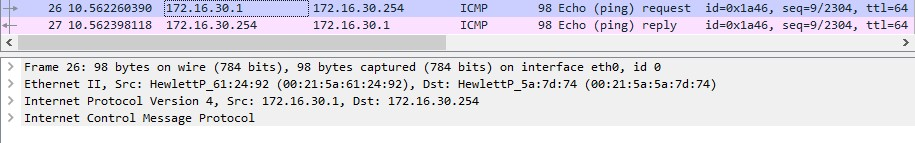
\includegraphics[width=\linewidth]{figure2}                                                      
    \caption{Pacote de Pedido}
    \label{fig:fig2}
\end{figure}

\begin{figure}[ht]
	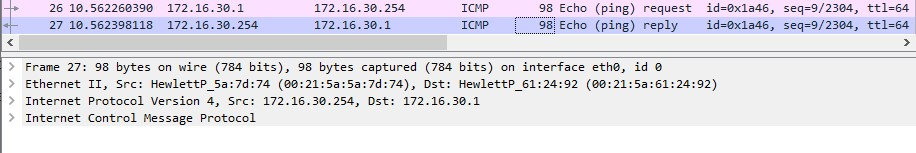
\includegraphics[width=\linewidth]{figure3}                                                      
    \caption{Pacote de Resposta}
    \label{fig:fig3}
\end{figure}

\begin{figure}[ht]
	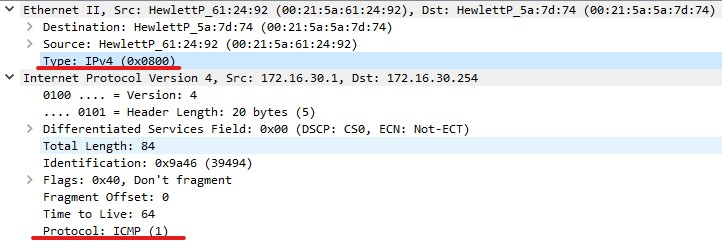
\includegraphics[width=\linewidth]{figure4}                                                      
    \caption{Campo Type Pacote ICMP}
    \label{fig:fig4}
\end{figure}

\begin{figure}[ht]
	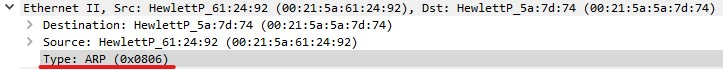
\includegraphics[width=\linewidth]{figure5}                                                      
    \caption{Campo Type Pacote ARP}
    \label{fig:fig5}
\end{figure}

\begin{figure}[ht]
	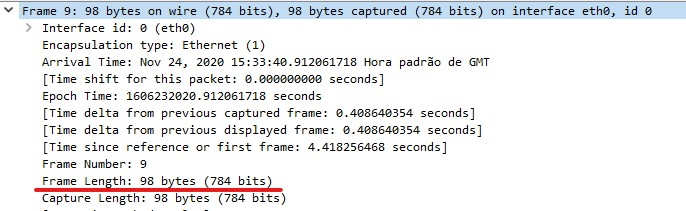
\includegraphics[width=\linewidth]{figure6}                                                      
    \caption{Tamanho de uma trama Recetora}
    \label{fig:fig6}
\end{figure}




\cleardoublepage
\phantomsection
\addcontentsline{toc}{subsection}{Aplicação Download}
\subsection*{Aplicação Download}

\subsubsection{download.c}
\lstinputlisting[language=c]{../download/src/download.c}

\subsubsection{getip.h}
\lstinputlisting[language=c]{../download/src/getip.h}

\subsubsection{getip.c}
\lstinputlisting[language=c]{../download/src/getip.c}

\subsubsection{connection.h}
\lstinputlisting[language=c]{../download/src/connection.h}

\subsubsection{connection.c}
\lstinputlisting[language=c]{../download/src/connection.c}

\subsubsection{Makefile}
\lstinputlisting[language=c]{../download/src/Makefile}



\end{document}